\documentclass{vgtc}                          % final 

%% to provide the the path and extension of a graphics file:
%% \includegraphics{diamondrule} is completely sufficient.
%%
\ifpdf%                                % if we use pdflatex
  \pdfoutput=1\relax                   % create PDFs from pdfLaTeX
  \pdfcompresslevel=9                  % PDF Compression
  \pdfoptionpdfminorversion=7          % create PDF 1.7
  \ExecuteOptions{pdftex}
  \usepackage{graphicx}                % allow us to embed graphics files
  \DeclareGraphicsExtensions{.pdf,.png,.jpg,.jpeg} % for pdflatex we expect .pdf, .png, or .jpg files
\else%                                 % else we use pure latex
  \ExecuteOptions{dvips}
  \usepackage{graphicx}                % allow us to embed graphics files
  \DeclareGraphicsExtensions{.eps}     % for pure latex we expect eps files
\fi%

%% it is recomended to use ``\autoref{sec:bla}'' instead of ``Fig.~\ref{sec:bla}''
\graphicspath{{figures/}{pictures/}{images/}{./}} % where to search for the images
\usepackage{accents}
\usepackage{microtype}                 % use micro-typography (slightly more compact, better to read)
\PassOptionsToPackage{warn}{textcomp}  % to address font issues with \textrightarrow
\usepackage{textcomp}                  % use better special symbols
\usepackage{mathptmx}                  % use matching math font
\usepackage{times}                     % we use Times as the main font
\renewcommand*\ttdefault{txtt}         % a nicer typewriter font
\usepackage{cite}                      % needed to automatically sort the references
\usepackage{tabu}                      % only used for the table example
\usepackage{booktabs}                  % only used for the table example
\usepackage{url}
%% OnlineID. Otherwise, you may safely leave it at ``0''.
\onlineid{0}

%% declare the category of your paper, only shown in review mode
\vgtccategory{Research}

%% allow for this line if you want the electronic option to work properly
\vgtcinsertpkg

%% In preprint mode you may define your own headline.
%\preprinttext{To appear in an IEEE VGTC sponsored conference.}

%% Paper title.

\title{M4: Final Submission}

%% This is how authors are specified in the conference style

%% Author and Affiliation (single author).
%%\author{Roy G. Biv\thanks{e-mail: roy.g.biv@aol.com}}
%%\affiliation{\scriptsize Allied Widgets Research}

%% Author and Affiliation (multiple authors with single affiliations).
%%\author{Roy G. Biv\thanks{e-mail: roy.g.biv@aol.com} %
%%\and Ed Grimley\thanks{e-mail:ed.grimley@aol.com} %
%%\and Martha Stewart\thanks{e-mail:martha.stewart@marthastewart.com}}
%%\affiliation{\scriptsize Martha Stewart Enterprises \\ Microsoft Research}

%% Author and Affiliation (multiple authors with multiple affiliations)
\author{Nicole Cherches\\
\scriptsize Matr. Nr.: 01506832
\and Alexander Gelb\\
\scriptsize Matr. Nr.: 01268620
\and Benjamin Neckam\\
\scriptsize Matr. Nr.: 01301917
\and Axynia Tokareva\\
\scriptsize Matr. Nr.: 01268620
}

%% A teaser figure can be included as follows, but is not recommended since
%% the space is now taken up by a full width abstract.
%\teaser{
%  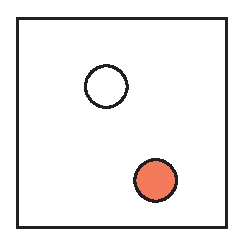
\includegraphics[width=1.5in]{sample.eps}
%  \caption{Lookit! Lookit!}
%}

%% ACM Computing Classification System (CCS). 
%% See <http://www.acm.org/about/class> for details.
%% We recommend the 2012 system <http://www.acm.org/about/class/class/2012>
%% For the 2012 system use the ``\CCScatTwelve'' which command takes four arguments.
%% The 1998 system <http://www.acm.org/about/class/class/2012> is still possible
%% For the 1998 system use the ``\CCScat'' which command takes four arguments.
%% In both cases the last two arguments (1998) or last three (2012) can be empty.

\CCScatlist{
  \CCScatTwelve{Visu\-al\-iza\-tion}{Visu\-al\-iza\-tion techniques}{}{};
  \CCScatTwelve{GAIA}{ESA}{}{}
}

%%%%%%%%%%%%%%%%%%%%%%%%%%%%%%%%%%%%%%%%%%%%%%%%%%%%%%%%%%%%%%%%
%%%%%%%%%%%%%%%%%%%%%% START OF THE PAPER %%%%%%%%%%%%%%%%%%%%%%
%%%%%%%%%%%%%%%%%%%%%%%%%%%%%%%%%%%%%%%%%%%%%%%%%%%%%%%%%%%%%%%%%

\begin{document}

%% The ``\maketitle'' command must be the first command after the
%% ``\begin{document}'' command. It prepares and prints the title block.

%% the only exception to this rule is the \firstsection command
\firstsection{Motivation}
\maketitle
On 19th December 2013 the "European Space Agency", ESA, launched  the "Gaia"-satellite to gather more information about our galaxy and create a three dimensional map out of it. Since then data like velocities, positions, errors, parallax and many more were collected of about 2 million stars. All together each star has 50 features in the data set which means the amount of entries is extremely high.\\
But working with such a huge dataset is not easy and most of the time not necessary because scientists only want to focus on a specific area of the galaxy. Therefore they only use subsets of the data. Now the idea was what happens if we take the whole data set and don't look into detail but see the "big picture" and try to find patterns, correlations, outliers or other interesting things.\\
This could be useful for scientists who are not sure which part of the data they want to explore and for example can focus only on the anomalies or other fascinating sections in the data set.

\section{Related Work}
What we first did, was searching for similar problems and finding out, what other visualizations looked like in this area. Most of the space visualizations we found online, were in 3d. Examples of them are the ESA Star Mapper\cite{starmapper} or 100000 stars\cite{chromeexperiment}. They both are 3d interactive simulations of the stellar neighbourhood.
We also found a 2d-visualization from the ESA, which visualizes the stars from the Gaia dataset\cite{gavs}.
But we couldn't find anything that has to do with correlations or patterns. All the existing visualizations were about showing the stars themselves with their exact location.
So we started prototyping and in the end we even used some of our first basic ideas in the end product of out system.
Then we tried to find existing visualization systems. In the VIS course we already learned about Tableau\cite{tableau}, which allows the user to import Data and create visualization plots based on it. And we also found out about a software named Glue\cite{glue}, which helps to create plots and analyze relationships between different data.
So we basically tried to create a mixture of both tools and started designing our own system.

\begin{figure}[h]
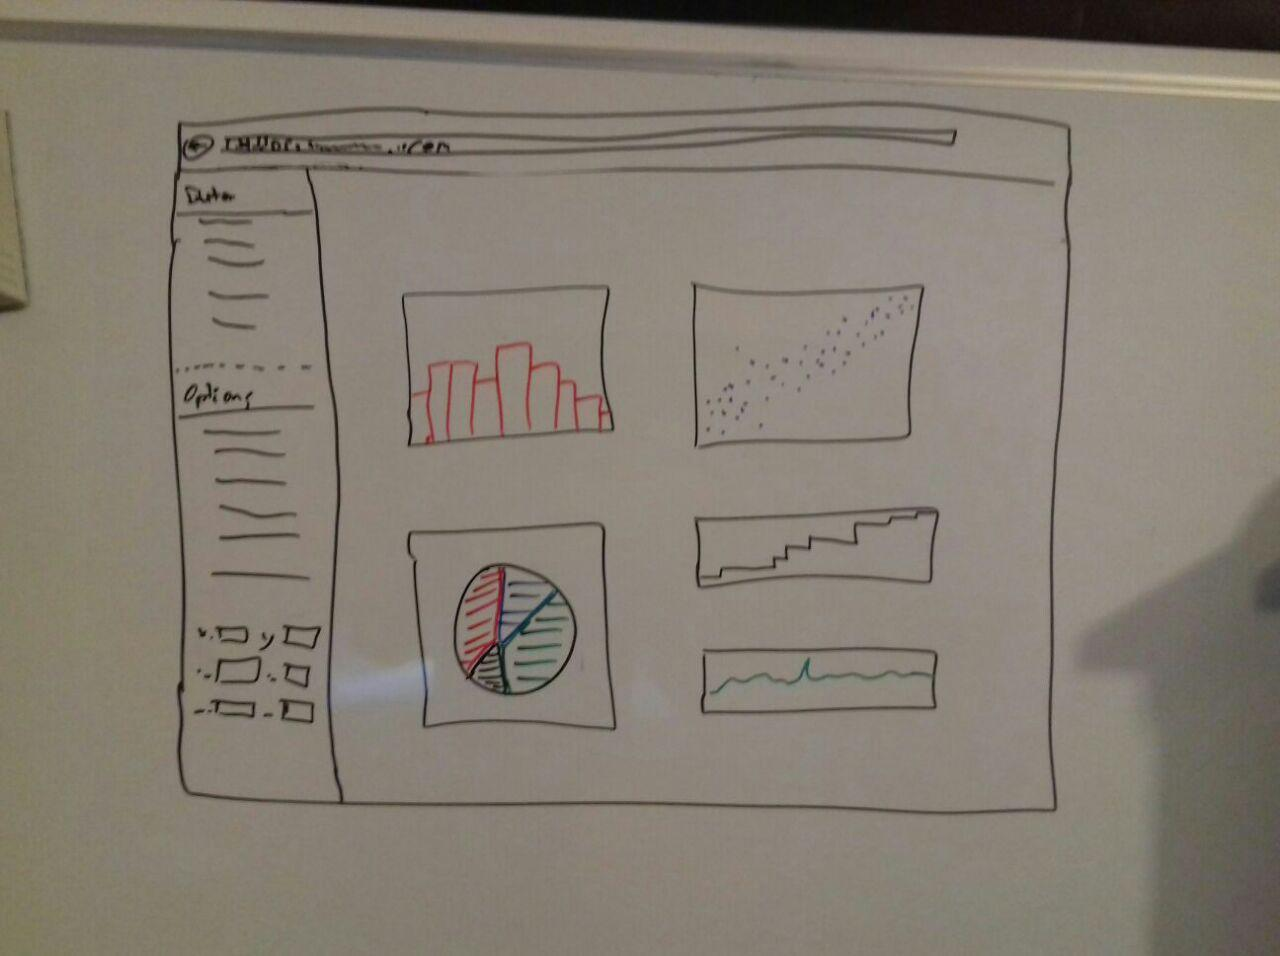
\includegraphics[width=0.5\textwidth]{Prototype1.jpg}
\centering
\caption{Lo-Fi Prototype of our user interface}
\end{figure}

Above is a picture, that shows how we imagined the visualization system at the beginning.
As we will see later in the end product, our Lo-Fi Prototype looks similar to our visualization system. We kept the sidebar, where the user has basic information about the data and can choose options on how the data will be presented. Also the diagrams and plots appear all on one screen so the user can see how they correlate.

\section{Approach}
When we first thought about our visualization design, we tried to think about our user. The system should help to see "the big picture" of a dataset and not only details. So, we thought about plots that could help us to realize that.

What we decided to do, was a Scatterplot Matrix: It really fits into our project, because we can see a whole grid filled with Scatterplots. This way, we can see all Correlations between selected columns of the Dataset.
The user has to choose a set of columns, he wants to analyse in the sidebar. The scatterplot has also histograms in the diagonal, so we can see the patterns even better.

Our system can also be used to compute histograms separately. Here the function creates bins for a specific column and shows how many entrys are in every bin. While hovering over the bars from our plot, we can also see the exact number of those entries.
The user can also set the bin size manually.

Then the system also provides a function to compute a Correlogram. For this, the user has also to select a set of columns. For these columns the function computes and displays the correlation coefficient. So it is easy to see how the different columns of a set are connected and if the user needs to analyse it further.

\section{Implementation}
The whole program was written in JavaScript combined with CSS. For the front-end we decided to use the toolkit "Bootstrap"\cite{bootstrap} which provides different templates so we needn't to spend to much time for designing the user-interface.\\
To visualize the data the JavaScript library "D3"\cite{d3} was used which offers the ability to let the user interact with the data.\\
\\
We encounters many problems which challenged us to implement things properly. One of the problems where to filter the data that all plots can be realized. We figured out that we just can't delete all the entries which contains a NULL or any other non valid values because this would reduce the data set to almost zero entries. Therefore we went through the documentation of the dataset and tried to figure out which features of the stars can be excluded and which not. Unfortunately we can not filter out all unnecessary values at the beginning , we have to do a "pre-filtering" to remove all non integer values and afterwards almost every function has to do their own filtering to adapt the data to their specific task.\\
To minimize the dataset we got the hint to have a look on "principal component analysis" which can help to reduce the dimensions. At the beginning we had the idea to implement a plugin\cite{pca} for D3 which processes the input data first and then work with it. But after implementing successfully we recognized that the produced result by the plugin was not that what we had in mind. It was built for datasets with less dimension than we have and therefore the performance was tremendously slow. So we focused on "DimStiller"\cite{dimstiller} and try to work with it. Basically it almost fulfilled our requirements but unfortunately it doesn't offer an API to connect it to our application. Due to time issues we weren't able to create pipeline where the input file is send to DimStiller which processes it and then send it back to our application where the user can work with a trimmed file. Although it is not realised yet we were curios how the result of DimStiller would look like and played around with it a little bit and decided to present the outcome here.\\
DimStiller's principal component analysis consists of five so called steps which happens consecutively. These are "Cull:Variance", "Data:Normalize", "Collect:Pearson", "Reduce:PCA" and "View:SPLOM". The first interesting and a little bit disappointment result appeared at "Collect:Pearson" which shows the correlation between the dimensions. It reduced the dimension from 52 to 28 dimension When we look on figure 2 we see that most of the dimensions are uncorrelated where we expected more correlation since the amount of data is enormous.\\
At the "Reduce:PCA" step one can choose interactively the final number of dimension via the user interface which is shown in figure 3. The problem here is that most dimensions get combined together and we are not sure how much and if there is an information loss. Due to this fusion the old names of the columns are discarded and get new names like "S4.D1" like we in figure 4 on the x axis. Furthermore we can see that picture concerning correlations haven changed, there are no or just slight correlation among the new dimensions.
\begin{figure}[h]
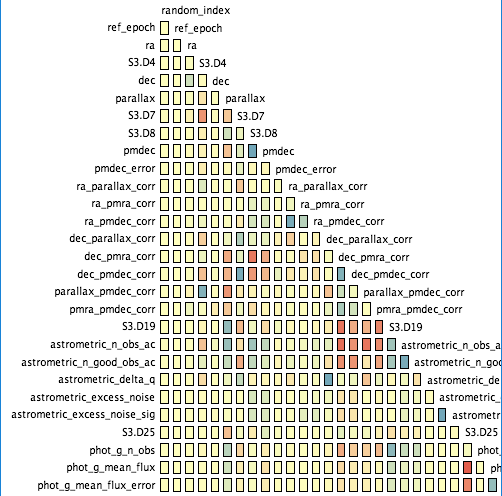
\includegraphics[width=0.5\textwidth]{pearsoncoeff.PNG}
\centering
\caption{Pearson coefficient where blue means positive correlation, yellow no correlation and red negative correlation}
\end{figure}
\begin{figure}[h]
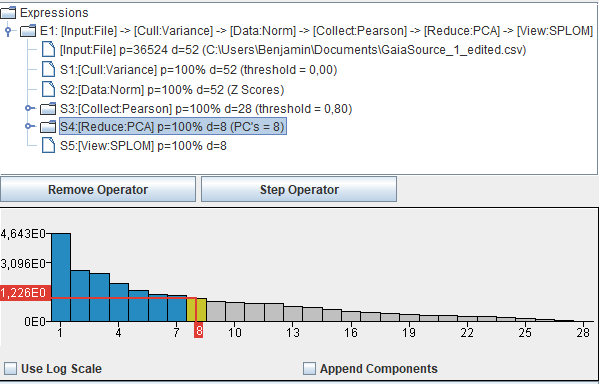
\includegraphics[width=0.5\textwidth]{pca.PNG}
\centering
\caption{PCA step}
\end{figure}
\begin{figure}
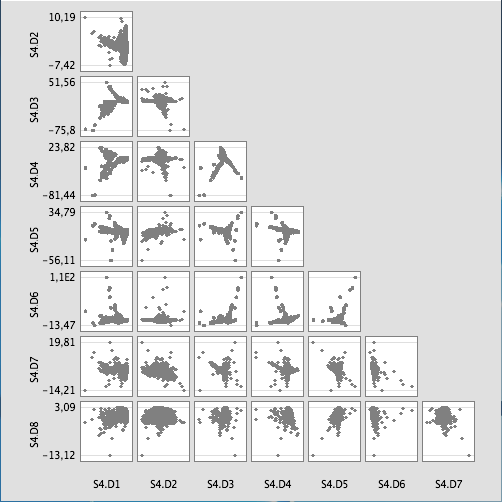
\includegraphics[width=0.5\textwidth]{splom.PNG}
\centering
\caption{Scatterplot matrix with reduced dimension to 8}
\end{figure}
\\
\\
As correlations are a major part in this project, we needed a way to compute correlations between columns in our big dataset.
So we used the formula for computing the correlation coefficient.\cite{corr}
\\
\\
$\rho_x{}_y$ = $\frac{\sum_{i=1}^n ((x_i-\overline{x}_n)(y_i - \overline{y}_n)}{\sqrt{\sum_{i=1}^n (x_i - \overline{x}_n)^2\sum_{i=1}^n(y_i - \overline{y}_n)^2}}$
\\
\\
This function is used for the correlogram and the scatterplot matrix.
The hard part about this, was that the formula is long and nested, so it was hard to compute in d3. Also it was difficult to debug this function because of the size of the dataset. Another challenge, was the right filtering of our data. For computing the correlation, we had to filter out empty entries or NaN values without modifying the data.
\section{Results}
The first thing the user will probably look on, is the information about the Gaia dataset. The name, number of rows and columns is displayed on the top left in the sidebar (Hier Bild). This sidebar contains also the Options: Here the user can choose the Columns he wants to analyse and chooses from all the columns in the Gaia Dataset. In this scenario our user wants to see the correlations between the columns "ra", "dec", "astrometric\_n\_obs\_al" and "l" (Hier Bild von Options und so). Then he presses "Plot" and the Scatterplot Matrix is displayed on the site (Hier Bild von mega nicer Scatter matrix). As said before now he can see all the columns on one look in one big view. The correlations between all the columns are computed and displayed as Scatterplots in the upper half of the Matrix, the values in the lower half. In the diagonal he can see histograms showing the distribution in the columns, also they have the column name in the title. When hovering over the bars he can read the exact value of the bar. Hovering over the correlation value displays the two column names, which where analysed. To clear the view, he can press "remove" and select new columns to plot. Or he just plots a new matrix underneath the old one.
\section{Discussion}
The main strength of our visualization project is, that the user has a fast overview, where he can see all the patterns and has "the big picture" of the dataset. With the Scatterplot Matrix he already can see how a set of columns correlates with each other, but that is not it: There are also histograms in the diagonal of the Matrix displaying the distribution of values in the chosen columns. The Scatterplots are displayed in the upper half and the correlation values in the lower half of the matrix. Also we implemented a regression line for the scatter plots. We are using tooltip for displaying furher information about plot objects and a filter, so the user can manually choose what he wants to see and ignore the rest. The visual strengths of our project are the simple design, because we only use few colours ("Less is more!"). 
The weakness of the design is the weak performance. The size of the dataset is a big problem, so it takes a lot of time to display the plots with so many points with Javascript and D3. Also we had a time management problem and couldn't achieve all that we wanted to do in this project (e.g. the PCA). 
\subsection{Lessons learned}
\subsubsection{Nicole Cherches}
There were a lot of things, I learned from the Gaia project. First of all, I would like to talk about the technical aspects: As this was my first visualization task, it was a whole new experience for me to work with d3 and Javascript. But the most important part is, that I learned how to work with a huge dataset and how to get the most out of it. We first tried to learn everything about it, also we realized that Astronomy is too complicated for us to understand. After our talk with Mr. Moeller, we then tried another approach: We did a data exploration task, which is all about exploring a huge dataset, we don't know much about.  
Another important part, I learned from this project, was working in a group on a big project. I learned a lot about coordination, planning and distributing tasks. This is also a good lesson, because collaboration with others is a necessary skill in computer science.
\subsubsection{Benjamin Neckam}
There were two things I will take out of this project.\\
First refers to the implementation and the chosen programming language. Basically I was not very used to JavaScript, to be more precisely I had no experience with it, but I was really impressed by "D3". The opportunities you have to visualize data is breathtaking and allows the programmer to choose over a wide variety of plot types. The only disadvantage that really falls into weight was the performance. If the dataset is bigger than, let's say, 100.000 entries it takes some time to calculate and plot the data and in our case the file contains more than ten times more entries. But all in all it was a very interesting and in my opinion very important for my future to work with JavaScript and "D3" and get deeper into this part of front end programming.\\
The second part is about the collaboration between the project group of the class and research group of another university. Until now all the projects at the university were from the teachers of the faculty itself but in this case the task was from the "Universitätssternwarte Wien". This means we had to arrange meetings with the project leader and a student which also is a member of the research group and talk about the task in detail and what the aim of this project is. It was fun and interesting to meet all these people but I recognized that even if there are not too many people involved it can easily happen that confusion arises. Like in our case, we started to focus on the wrong details and parts and had to "restart" our project. Therefore I would say communication is the most important part in a project, especially if it is a collaboration of two or more groups, I guess this is the biggest lesson I learned from the project. 
\section{Separation of Tasks}
Nicole Cherches: Report, Corrrelation analysis\\
Alexander Gelb: Scatterplots, Regression line\\
Benjamin Neckam: Report, Principal Component Analysis\\
Axynia Tokareva: Histograms, insert correlations in scattermatrix, Tooltips, Scales
\bibliographystyle{unsrt}
\bibliography{reference}

\end{document}